\documentclass[onecolumn, draftclsnofoot,10pt, compsoc]{IEEEtran}
\usepackage{graphicx}
\usepackage{url}
\usepackage{setspace}
% Set backend as appropriate
\usepackage[style=ieee,backend=biber]{biblatex}
\usepackage{geometry}
\bibliography{references}
\geometry{textheight=9.5in, textwidth=7in}

\def \CapstoneTeamName{		Enteral Feeding Calculator Team}
\def \CapstoneTeamNumber{		60}
\def \GroupMemberOne{			Alison Jones}
\def \GroupMemberTwo{			Parker Okonek}
\def \CapstoneProjectName{		Volume-Based Enteral Feeding Calculator}
%\def \CapstoneSponsorCompany{	Company, Inc}
\def \CapstoneSponsorPerson{		Dr. Judy Davidson}

\def \DocType{
				Winter End-Of-Term Report
				}
			
\newcommand{\NameSigPair}[1]{\par
\makebox[2.75in][r]{#1} \hfil 	\makebox[3.25in]{\makebox[2.25in]{\hrulefill} \hfill		\makebox[.75in]{\hrulefill}}
\par\vspace{-12pt} \textit{\tiny\noindent
\makebox[2.75in]{} \hfil		\makebox[3.25in]{\makebox[2.25in][r]{Signature} \hfill	\makebox[.75in][r]{Date}}}}
% 3. If the document is not to be signed, uncomment the RENEWcommand below
%\renewcommand{\NameSigPair}[1]{#1}

%%%%%%%%%%%%%%%%%%%%%%%%%%%%%%%%%%%%%%%
\begin{document}
\begin{titlepage}
    \pagenumbering{gobble}
    \begin{singlespace}
        \hfill 
        \par\vspace{.2in}
        \centering
        \scshape{
            \huge CS Capstone \DocType \par
             \large\GroupMemberOne\par
            \large\GroupMemberTwo\par
            {\large\today}\par
        }
        \vfill
    \begin{abstract}
        The enteral feeding calculator is an open-source, windows desktop application written in C\# and based off of the .NET framework.
        The purpose of the calculator is to provide an easy to use, dependable, and accurate replacement for enteral feeding paper calculation tables.
        Development of the calculator has undergone many changes in user interface and target platform requirements with inconclusive results from different nurse groups and issues establishing integration with the preferred patient database software.
        
        The calculator still lacks error checking and data validation in its run-time and file loading operations and lacks a polished user interface to maximally ease nurse use.
    \end{abstract}
    \end{singlespace}
    \end{titlepage}
    \clearpage
\pagenumbering{arabic}
\section{Overview}
The enteral feeding calculator project is an implementation of the enteral feeding catch-up table designed by Dr. Heyland and managed by Judy Davidson.
The main goal of the project is replace the manual method of calculating volumetric enteral feeding rates with an automated, digital method with less user error, higher accuracy results, and faster calculation time.
The application accounts for missed feeding times and provides the best possible new feeding rate.
The target platform for development is a windows-based desktop OS.
The purpose of it is to increase efficiency and effectiveness among nurses during the tube feeding process.

Design of the user experience and interface is oriented towards a low barrier of entry visual style with minimal complexity presented for user input to reduce errors.
\section{Current State}
The current status of the project appears to be on track with initial expectations, however stretch goals may not be met. Stretch goals will be outlined in the 'Future Work' section.

The project currently supports much of its planned functionality.
Feeding rates for patients are currently able to be generated with higher accuracy with the paper table.
The enteral calculator allows for users to add feed start and stop times adjusted to the 24 hour window from current day daily start time to next day's daily start time and for users to remove all feeding times as needed to correct patient timeline data.
All patient information can now be configured as well: patient id is adjustable from the change name dialog, daily start time is editable from the patient configuration dialog, feeding type and default feed rates are set from the patient configuration dialog in addition to daily volume goal rate and (if needed) maximum feed rate override.

Patient information can be saved to a file or loaded from a file to manage multiple patients or to ensure that the patient's information is not lost across nurse shifts or sudden power loss.
Currently patient information is not adjusted when the internal clock detects that the reset time has been reached, but the reset time is used when determining which data in a timeline file to keep on file load, ensuring that hours outside of the nurse's shift window and the feeding schedule are not listed.

\begin{figure}[htp]
    \centering
    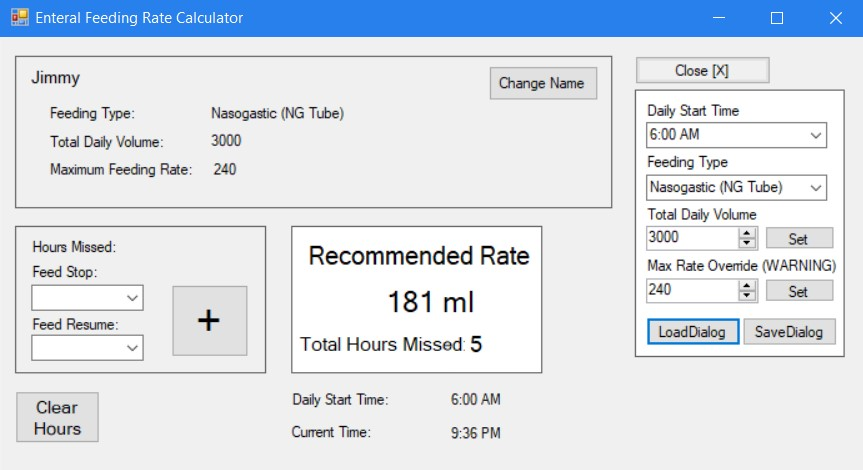
\includegraphics[width=17cm]{betainterface}
    \caption{Beta Interface}
    \label{fig:Beta}
\end{figure}

\begin{figure}[htp]
    \centering
    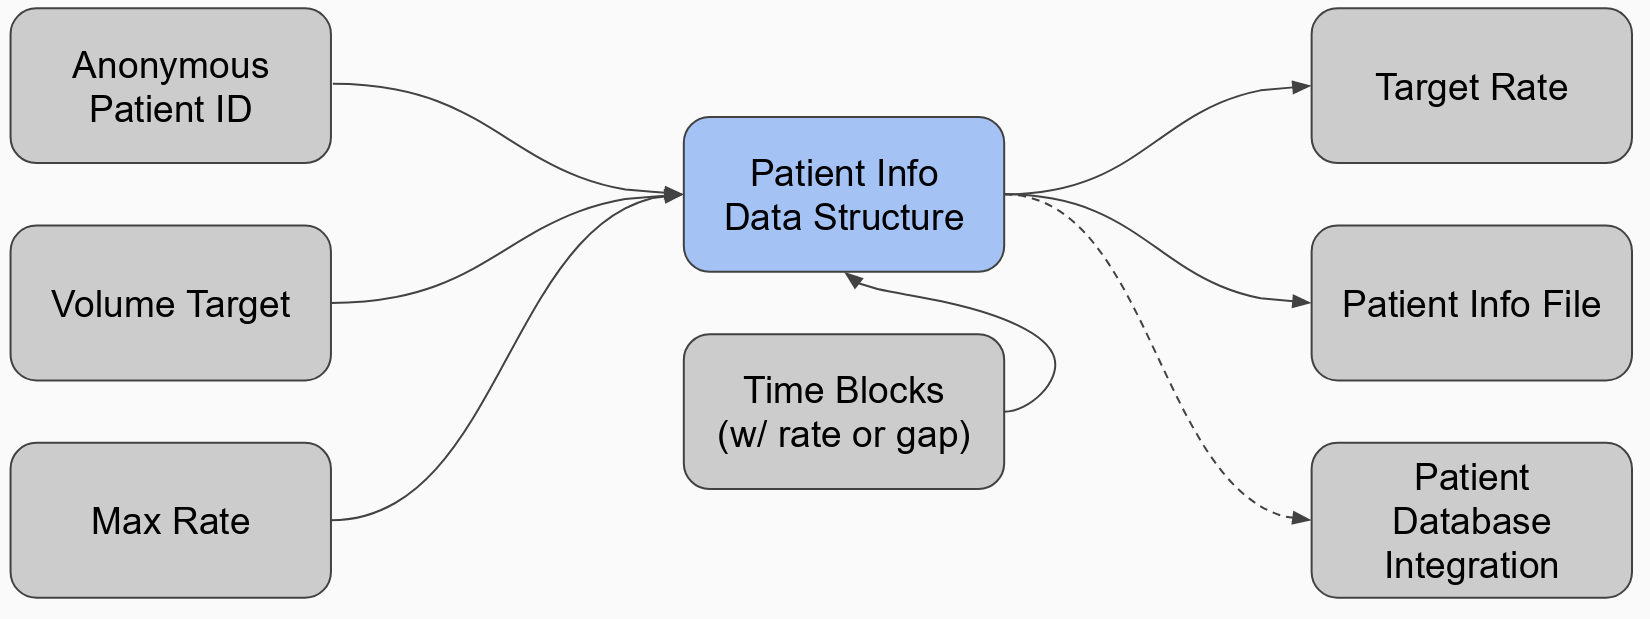
\includegraphics[width=17cm]{patientinfo}
    \caption{A patient information class object is composed of several pieces of data collected from nurse input which is maintained persistently in application run-time and patient data files. The patients missed and feed times are also maintained in this object.}
    \label{fig:Patient Info Flowchart}
\end{figure}

\begin{figure}[htp]
    \centering
    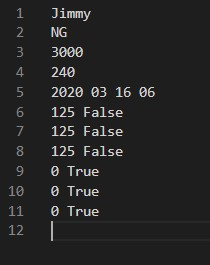
\includegraphics[width=6cm]{patientexample}
    \caption{Patient files contain all the information needed to determine a patient's goal rate over the course of a shift in addition to an anonymous patient identifier and a timestamp of the daily reset time of the date when the file was saved.}
    \label{fig:Patient File Example}
\end{figure}

\begin{figure}[htp]
    \centering
    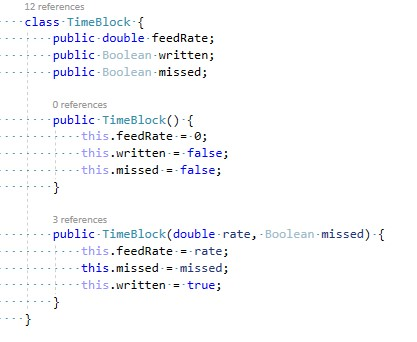
\includegraphics[width=13cm]{timeblock}
    \caption{Class definition for time blocks. These data structures are used to compose a complete patient timeline which can be manipulated by the user interface, saved to a file, and combined in order to tabulate patient feeding rates and total hours missed.}
    \label{fig:Timeblock}
\end{figure}

\begin{figure}[htp]
    \centering
    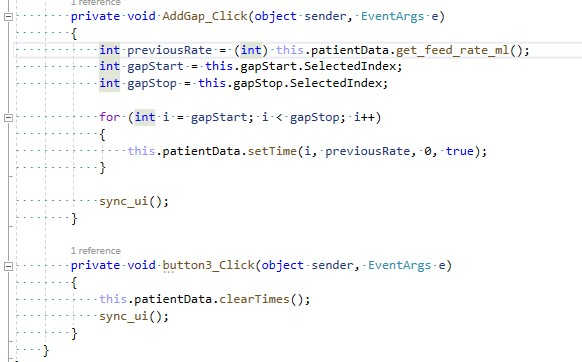
\includegraphics[width=16cm]{buttoncode}
    \caption{Adding a gap of missed times to the patient info timeline is activated by an event from the user interface. The function enters every time between in the gap time block by time block and then calls the standardized call to update the UI values to changes in the patient info object.}
    \label{fig:ButtonCode1}
\end{figure}


\begin{figure}[htp]
    \centering
    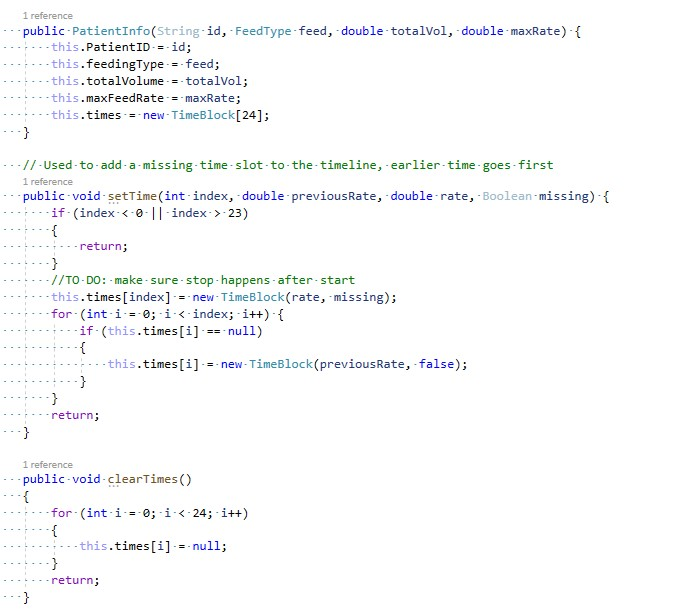
\includegraphics[width=18cm]{code2}
    \caption{Code within the PatientInfo.cs file. This includes the structure for the Patient file being exported which contains patient name, feeding type, daily total volume, maximum feeding rate, and the time blocks for the 24hr day cycle. The two functions included help manage the data being stored as time blocks. These time blocks determine when a patient was or wasn't fed. The first function is setTime which sets an index in the times array to the appropriate rate and status of the patient during that hour. The second function, clearTimes, is used to reset the times array if any mistakes are mad or if a nurse wants to clear out a patient's data for the day. This would also be called at our daily reset time.}
    \label{fig:HoursData}
\end{figure}

\section{Future Work}
There are still a few issues that need to be addressed in the calculator. While we have personally tested the app and conducted user tests, there are still likely bugs! We should conduct a few more stress tests and scenarios to verify that errors cannot be made. This is especially important if the app is to be used in any medical context.This means that we can be expected to conduct a few more user tests before this project is finished.
\newline 
In addition to usability in the functional sense, we also want to improve it in the scope of interaction and appearance. Our layout has drastically changed over each update as new features are added and unnecessary ones are removed. This can be anything from button layout and interaction flow to color, readability, and scaling. This means that during user testing for bugs we should also allow some time for user feedback on the UI's appearance and feel. We should go through at least one or two more reviews with a client or user (audience member) before finalizing the project. With the time remaining this will likely include one with our clients and another with a group of nurses. Smaller meetings with the client will be held to get feedback, but at least one more full review and test should be held with the client as well. 
\newline
Stretch goals for future development include the integration of titration and cross platform implementation. Titration is a method often used when adjusting a patient's feeding rate. While this is more important when increasing feeding rate, it can be used for decreasing the rate as well. We will only need to add it in the context of increasing feeding rate. Titrating a feeding means that the feeding speed is not increased all at once, but instead, small adjustments are made over time. This helps avoid any pain, discomfort, or complications when increasing rate. 
\newline
Platform of choice was cause for debate throughout the entire development of this application. We eventually settled on a Windows application, however there are many areas that the client and other nurses viewed as potential candidates for this project.
\newline
The open source goals of the project will be retained by continuing hosting of the code publicly on Github.
Many of the details of the Github hosting are to be determined, the main maintainers of the the repository after the conclusion of our capstone project is currently unknown, as well as where the compiled releases of the application will be listed with Github being a prime candidate for this as well.

\section{Problems}
Many problems in the development of the application were derived from inconclusive user studies and mixed ideas on the target platform.
Our team underwent many user studies with different groups of nurses local to the Corvallis area and the nurses available to our clients in University of California San Diego Health.
As part of these user studies we showed the nurses paper prototypes of our user interfaces and we questioned the nurses on the platforms available to them in a hospital setting.
The nurses raised several concerns over maintaining patient confidentiality and notifying incoming nurses of needed adjustments in enteral feeding rate across shift changes.

These user studies resulted in an inconclusive set of conflicting feedback from different nurse groups.
Each nurse group had a different requirement or enteral feeding rate data entry: some nurse groups believed the entry should be based off of hours missed total, while other groups believed the entry should be based off of a a collection of start and end time pairs. Due to all of these discrepancies, we did make adjustments in order to best include as many needs as possible including customization of most fields. 

Aside from user interface indecision, nurses were agreed on one point: the application should not be based off of iOS or Android, but should instead be web focused as an integrated service to the most common patient database management system, EPIC.
EPIC integration was our goal entering winter term, with our current program base serving as an example of what an EPIC integrated app would look and act like without having access to EPIC integration or services.
However, our goal of EPIC integration was cancelled when we were informed of security concerns of us integrating into EPIC.
This response from the EPIC team made it clear to both our clients and our team that EPIC integration would not be supported on their end and that development could not continue in this direction; after this, our development again shifted focus to a Windows Desktop environment.

\section{Solutions}
Our team resolved the interface indecision by planning for a compromise between the two systems.
We have begun to implement a visual representation of the timeline that will allow nurses to click on individual time blocks instead of specifying them with drop-down entry.
This interface will allow for nurses to visually conceptualize the timeline while changing its feeding rate values as well as adding and deleting feeding rate times and adding blocks of missing feeds.

The issues with the platform and EPIC integration were resolved by migrating the final platform of the project to our platform used to demonstrate basic functionality that could be achieved with the application.
Our chosen platform was C\# as a development language with windows as the targeted development platform.
Additionally we used the .NET framework and Windows Form App library to create our user interface and integration with the Windows operating system.
This platform also allows for a level in integration with other web platforms in the future which take a different approach than EPICs service.
The application is extensible and could be used to integrate with RESTful apis, unlike EPICs integration which requires the application to be written entirely within the customer's instance of EPIC and their proprietary environment.

\section{Research}
Multiple reviews and meetings with both our clients and nurses have been held in order to grab lots of information providing a full image of what the target audience wants in our application. There have been many differing opinions on how we should go about the development of this app. The initial request was for a phone app since our client's team of nurses plan to have iPhones available for work tasks. The main problem with this was that while this is likely the best solution (and most convenient) for our client, it isn't necessarily the best in the long term or for the majority of hospitals. Along with creating an app, our client had a goal for this tool to be open source and available to as many people as possible. A phone app would be more portable, but not as universally used in hospitals. One set of nurses we interviewed even mentioned that they don't allow phones when working. To pull even further away from phone apps was the idea of integration, specifically with EPIC. Our client was wonderful enough to try expanding our tool's use by integrating it with a commonly used patient management system. Discussions with people who work on EPIC showed that linking to a web application may be the easiest mode of integration, however hosting would cost money. We ultimately settled with a desktop app. Despite being incompatible with iPhones and less portable than a web app, this form of application would be compatible with a substantial number of computers in hospitals (any Win 10 machines) and could be easily distributed. This form would also be isolated and thus secure from an external viewpoint. There is no need to store or send sensitive data. This interface choice was eventually approved by our client and had a backing from local nurses. There were a few meetings after deciding this platform that swayed our choice, however by the time these happened we were far enough into the project that it would be counterproductive to backtrack onto another platform. Some user input during research also requested clearer notifications for resets and data changes. More research must be done to verify that the new alerts we have added are enough but not too much. Our application has had some major overhauls since the last user tests were conducted so we will need to schedule a few for our current (beta) interface. 

\end{document}
